\documentclass[aspectratio=169]{beamer}

%\includeonlyframes{current}

\usepackage[utf8]{inputenc}
\usepackage[american]{babel}
\usepackage{amsmath,amsthm}
\usepackage{unicode}
\usepackage{array,tabularx}
\usepackage{ifthen}
\usepackage{tikz}
\usetikzlibrary{matrix,decorations,decorations.text,calc,arrows,snakes,shapes,positioning}
\usepackage{tikzsymbols}
\usepackage[backend=biber,citestyle=authoryear-comp,bibstyle=beamer,doi=false,isbn=false,url=true,maxnames=10]{biblatex}
\bibliography{refs}

\usepackage{ulem}

\mode<presentation>{%
  \usetheme{ibm}
}

\newcommand{\C}{ℂ}
\newcommand{\R}{ℝ}
\newcommand{\Z}{ℤ}
\newcommand{\N}{ℕ}
\newcommand{\Q}{ℚ}
\newcommand{\F}{\mathbb{F}}
\renewcommand{\P}{\mathbb{P}}
\renewcommand{\O}{\mathcal{O}}
\newcommand{\tildO}{\mathcal{\tilde{O}}}
\newcommand{\poly}{\operatorname{poly}}
\newcommand{\polylog}{\operatorname{polylog}}
\newcommand{\End}{\operatorname{End}}
\newcommand{\Hom}{\operatorname{Hom}}
\newcommand{\Gal}{\operatorname{Gal}}
\newcommand{\chr}{\operatorname{char}}
\newcommand{\Cl}{\operatorname{Cl}}
\newcommand{\GL}{\operatorname{GL}}
\renewcommand{\a}{{\mathfrak{a}}}
\renewcommand{\b}{{\mathfrak{b}}}
\newcommand{\p}{{\mathfrak{p}}}
\newcommand{\q}{{\mathfrak{q}}}
\newcommand{\g}{{\mathfrak{g}}}
\newcommand{\G}{{\mathcal{G}}}
\newcommand{\E}{{\mathcal{E}}}
\newcommand{\cyc}[1]{{〈 #1 〉}}
\newcommand{\ord}{\operatorname{ord}}
\newcommand{\mat}[1]{\left(\begin{smallmatrix}#1\end{smallmatrix}\right)}
\newcommand{\from}{\overset{\$}{\leftarrow}}

\newcommand{\bl}[1]{\textcolor{blue}{#1}}
\newcommand{\rd}[1]{\textcolor{red}{#1}}
\newcommand{\gr}[1]{\textcolor{green}{#1}}
\newcommand{\og}[1]{\textcolor{orange}{#1}}

\definecolor{light blue}{RGB}{0,102,204}

\newcommand{\myedge}[3]{
  \draw[#3] (360/\crater*#1 : \diam) to[bend right] (360/\crater*#2 : \diam);
}
\newcommand{\sk}[4]{
  \draw[very thick,blue]   (0,0) -- (0,#1);
  \draw[very thick,red]    (1,0) -- (1,#2);
  \draw[very thick,green]  (2,0) -- (2,#3);
  \draw[very thick,orange] (3,0) -- (3,#4);
}
\newcommand{\axes}[4]{
  \clip (#1,#3) rectangle (#2,#4);
  \draw [thin, gray, -latex] (#1,0) -- (#2,0);% Draw x axis
  \draw [thin, gray, -latex] (0,#3) -- (0,#4);% Draw y axis
}
\pgfkeys{/lattice/.code n args={4}{\tikzset{cm={#1,#2,#3,#4,(0,0)}}}}
\newcommand{\lattice}[2]{
  \draw[style=help lines,dashed] (#1-1,#1-1) grid[step=1] (#2+1,#2+1);
  \foreach \x in {#1,...,#2}{
    \foreach \y in {#1,...,#2}{
      \node[draw,circle,inner sep=2pt,fill] at (\x,\y) {};
      % Places a dot at those points
    }
  }
}

\newenvironment<>{goodblock}[1]{%
  \begin{actionenv}#2%
      \def\insertblocktitle{#1}%
      \par%
      \mode<presentation>{%
        \setbeamercolor{block title}{fg=green!60!black,bg=green!50!white}
       \setbeamercolor{block body}{bg=green!20!white}
     }%
      \usebeamertemplate{block begin}}
    {\par\usebeamertemplate{block end}\end{actionenv}}
\newenvironment<>{mehblock}[1]{%
  \begin{actionenv}#2%
      \def\insertblocktitle{#1}%
      \par%
      \mode<presentation>{%
        \setbeamercolor{block title}{fg=yellow!50!black,bg=yellow!50!white}
       \setbeamercolor{block body}{bg=yellow!20!white}
     }%
      \usebeamertemplate{block begin}}
    {\par\usebeamertemplate{block end}\end{actionenv}}
\newenvironment<>{badblock}[1]{%
  \begin{actionenv}#2%
      \def\insertblocktitle{#1}%
      \par%
      \mode<presentation>{%
        \setbeamercolor{block title}{fg=red!60!black,bg=red!50!white}
       \setbeamercolor{block body}{bg=red!20!white}
     }%
      \usebeamertemplate{block begin}}
    {\par\usebeamertemplate{block end}\end{actionenv}}


../share/isographs.tex

\title{SQIsign, the number theorists' great crypto heist}
\author{Luca De Feo}
\date[June 28, 2023, RTCA 2023]{June 28, 2023\\
   Recent Trends in Computer Algebra 2023}
\institute{IBM Research Zürich}

\begin{document}

\frame[plain]{\titlepage}

%%

\begin{frame}{Hi, it's me!}
  \begin{itemize}
  \item<+-> Started into research working on (essentially) \emph{counting
      points of elliptic curves}.
  \item<+-> Very quickly got distracted by \emph{efficient computations in
      finite fields}.
  \item<+-> I was using \emph{Magma and NTL}. Got very
    frustrated with Magma's finite fields.
  \item<+-> Never counted a single point, ended up with a thesis on
    \emph{computing isogenies of elliptic curves} for the sake of
    computing them.
  \item<+-> Postdoc in Waterloo. David Jao shows me his new cute idea to
    make an encryption system out of \emph{isogenies of supersingular
      curves}, asks me if I can make it fast.
  \item<+-> I could.
  \item<+-> That's also when I started seriously working with
    \emph{Sage and Flint}.
  \item<+-> Went back to France and finite fields, but never stayed
    too far from elliptic curves.
  \end{itemize}
\end{frame}

%%

\begin{frame}{\dots continued}
  \begin{description}
  \item[2015--2019]<+-> Member of \emph{OpenDreamKit}, I start digging
    into the gory depths of Sage \& friends.
  \item[2016]<+-> Our little encryption system \emph{(SIDH/SIKE)}
    starts getting more attention than expected.
  \item[2017]<+-> People start talking a lot about \emph{post-quantum
      cryptography}, for some reason think isogenies are the way
    forward.
  \item[2018--now]<+-> I become more interested in making new
    cryptography, end up inventing a few more \emph{isogeny-based
      systems}. Some are even sort of efficient.
  \item[2019]<+-> Move to IBM Research. I guess I'm a cryptographer,
    now.
  \item[June 2022]<+-> SIKE is selected for the 4th round of NIST's
    competition.
  \item[July 2022]<+-> \dots
  \end{description}
\end{frame}

%%

\begin{frame}[plain]
  \centering
  \begin{tikzpicture}[remember picture,overlay]
    \node[at=(current page.center)] {
      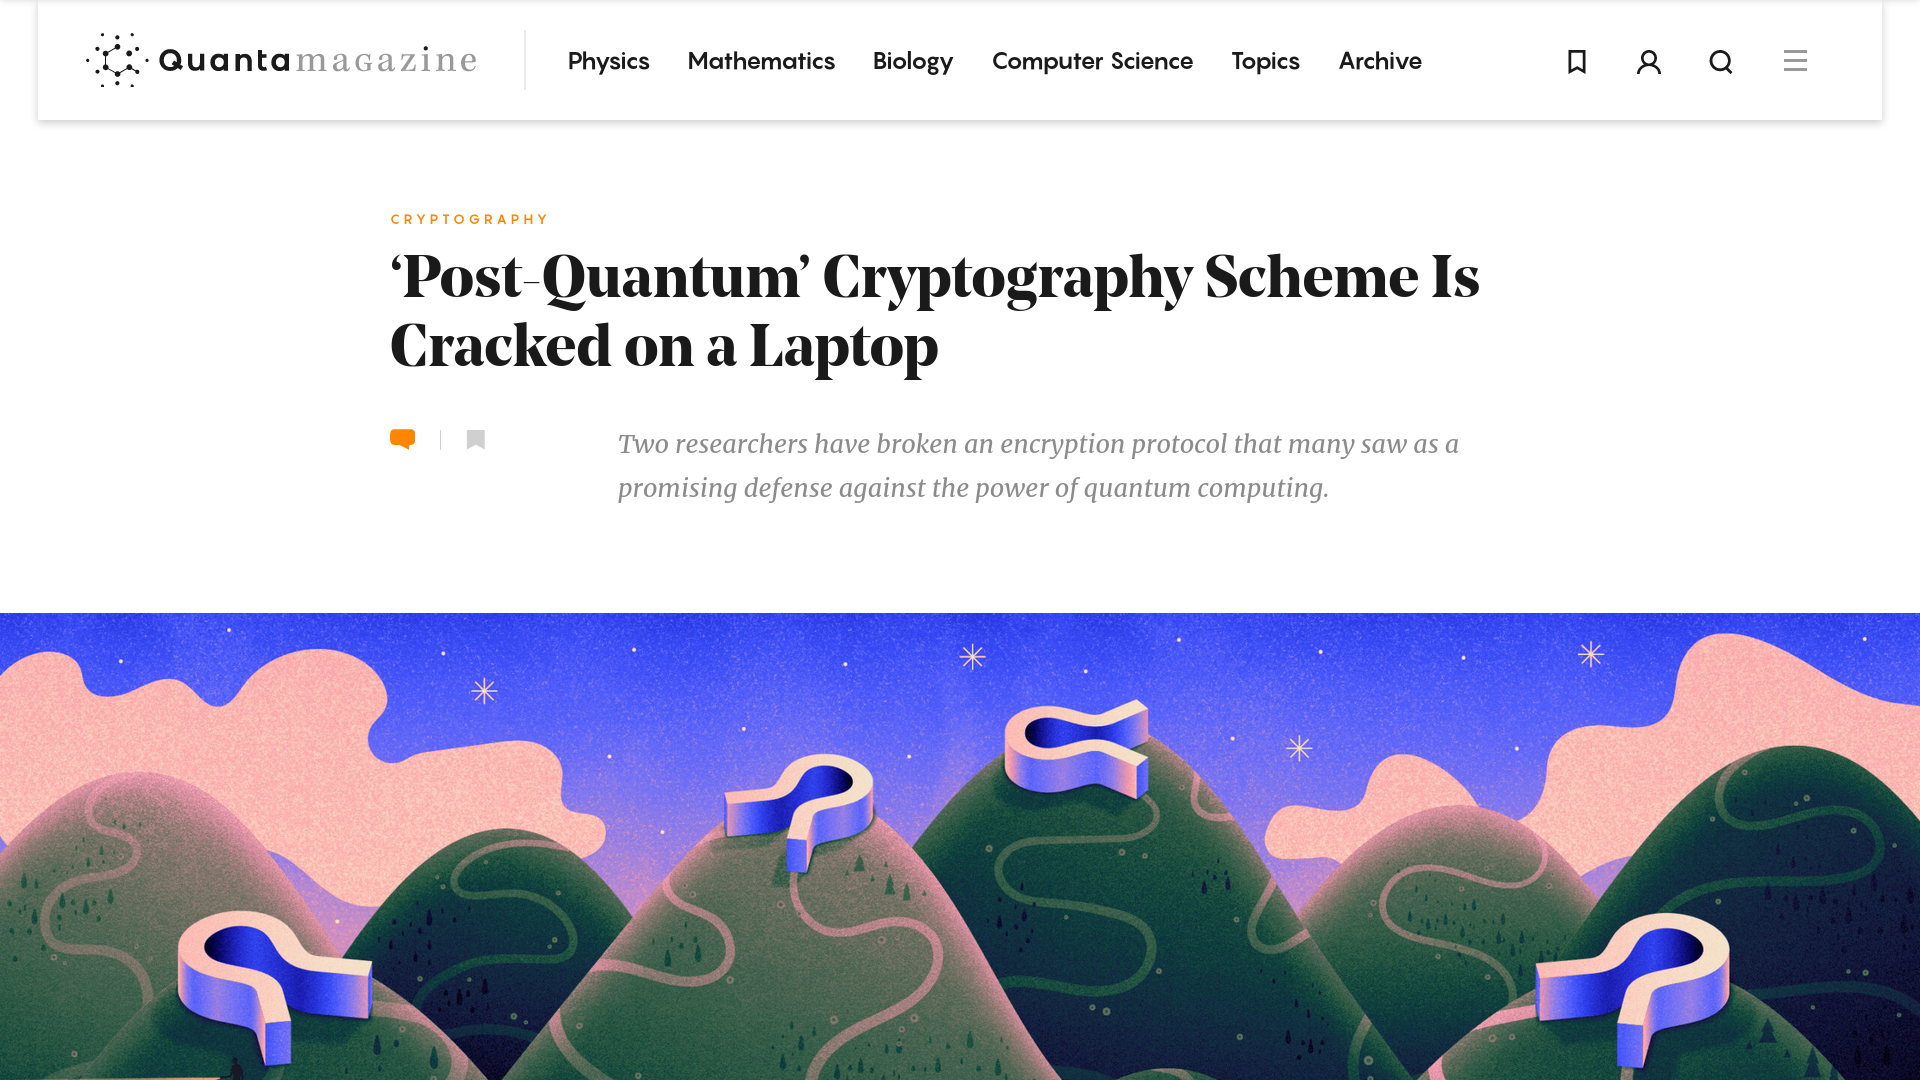
\includegraphics[width=\paperwidth]{quantamag-sike.png}
    };
  \end{tikzpicture}
\end{frame}

%%

\begin{frame}{Why am I here today?}
  \Large
  \begin{itemize}
    \setlength{\itemsep}{3em}
  \item<+-> To share my experience implementing cryptography.
  \item<+-> To show you some cool maths.
  \item<+-> To know if msolve can run on a quantum computer.
  \end{itemize}
\end{frame}

%%

\frame[plain]{
  \begin{beamercolorbox}[sep=2em,left,wd=\paperwidth,ht=\paperheight,dp=0px]{palette tertiary}
    \centering
    \usebeamerfont{title}{Implementing Crypto}
    \vspace{0.4\paperheight}
  \end{beamercolorbox}
}

%%

\begin{frame}{A different game\dots}
  \begin{itemize}
    \setlength{\itemsep}{1em}
  \item Quite the \emph{opposite of general purpose}.
  \item Old salty dogs write \emph{C/C++}, cool kids write \emph{Rust}.
  \item Must fit in all sorts of \emph{strange platforms} (e.g.,
    smartphones, smartcards).
  \item The more code, the more trouble.
  \item Code must be easily \emph{auditable}.
  \item Misunderstanding the spec of a function can be fatal!
  \item \emph{Randomness} is a pain. Always.
  \end{itemize}
\end{frame}

%%

\begin{frame}{and yet, some familiarity\dots}
  \begin{columns}
    \begin{column}{0.6\textwidth}
      \begin{itemize}
        \setlength{\itemsep}{2em}
      \item Most code \emph{open source}. Good for auditability.
      \item Mostly developed by volunteers on their spare time.
      \item E.g.: OpenSSL (50\% market share) has only 2 full-time
        developers and 1M\$ budget.
      \end{itemize}
    \end{column}
    \begin{column}{0.4\textwidth}
      \centering
      \includegraphics[height=0.9\textheight]{xkcd-dependency}
    \end{column}
  \end{columns}
\end{frame}

%%

\begin{frame}{with some unique rules: Secure coding}
  \begin{itemize}
    \setlength{\itemsep}{2em}
  \item Avoid external dependencies as much as possible.
  \item Dynamic memory allocation shunned.
  \item \emph{Constant time:} running time must be independent from
    secrets.
  \item Code must be robust against errors (incl.\ cosmic rays).
  \end{itemize}
\end{frame}

%%

\begin{frame}{Computer algebra in pre-quantum crypto}
  \begin{block}{RSA}
    \begin{itemize}
    \item Multi-precision integers.
      \begin{itemize}
      \item Bit-sizes: 2048, 3072, 4096, 7680, 15360, \dots
      \end{itemize}
    \end{itemize}
  \end{block}

  \begin{block}{ECC}
    \begin{itemize}
    \item Arithmetic in $\Z/p\Z$.
      \begin{itemize}
      \item Bit-sizes: 256, 384, 512, \dots
      \end{itemize}
    \item Elliptic curve addition/duplication formulas
    \end{itemize}
  \end{block}
\end{frame}

%%

\begin{frame}{Computer algebra in post-quantum crypto}
  \begin{block}{CRYSTALS -- Kyber/Dilithium (lattice based)}
    \begin{itemize}
    \item Arithmetic in $(\Z/p\Z)[X]/(X^{256} + 1)$,
      \begin{itemize}
      \item where $p=3329,8380417$ (FFT friendly).
      \end{itemize}
    \item Matrix operations
      \begin{itemize}
      \item from $2\times 2$ to $8\times 7$.
      \end{itemize}
    \end{itemize}
  \end{block}

  \begin{block}{Multi-quadratics (UOV, etc.)}
    \begin{itemize}
    \item Multivariate dense polynomials over $\Z/p\Z$.
    \item Linear system solving.
      \begin{itemize}
      \item e.g.: $p=31$, dimension $\approx 50 \times 150$.
      \end{itemize}
    \end{itemize}
  \end{block}
\end{frame}

%%

\begin{frame}{Computer algebra in post-quantum crypto}
  \begin{block}{Code based (McEliece, etc.)}
    \begin{itemize}
    \item Matrices over binary fields
      \begin{itemize}
      \item dimensions in the hundreds to thousands.
      \end{itemize}
    \item (List) decoding algorithms.
    \end{itemize}
  \end{block}

  \begin{block}{SIKE (isogeny based)}
    \begin{itemize}
    \item Arithmetic in $\F_p[i]/(i^2+1)$
      \begin{itemize}
      \item bit-sizes $434, 503, 610, 751$
      \end{itemize}
    \item Elliptic curve arithmetic.
    \item Isogeny formulas.
    \item Isogeny composition.
    \item Optional: Weil pairing, discrete logs in
      $C_{2^e}\times C_{2^e}$.
    \end{itemize}
  \end{block}
\end{frame}

%%

\begin{frame}{SQIsign}
  \centering
  \begin{tikzpicture}
    \node[draw] (bigint) at (0,2.5) {\emph{BigInts}};
    \node[draw] (quat) at (3.6,2.5) {
      \parbox{4cm}{
        \emph{Quaternions}\\[1ex]
        (modular) Integer matrices, kernels, lattices,
        orders (maximal, Eichler),
        LLL, HNF, Howell form, \dots
      }};
    \node[draw] (klpt) at (9,2.5) {
      \parbox{4cm}{
        \emph{KLPT}\\[1ex]
        Diophantine equations (Cornacchia), norm equations, \dots
      }};
    \node[draw] (gf) at (2,-2.5) {\emph{$\F_{p^2}$}};
    \node[draw] (ec) at (6,-2.5) {
      \parbox{4cm}{
        \emph{Elliptic curves}\\[1ex]
        Isogenies, Weil pairing, discrete logs, \dots
      }};
    \node[draw] (i2i) at (12,0) {
      \parbox{3cm}{\centering
        \emph{Ideal $\leftrightarrow$ Isogeny translation.}
      }};

    \draw[-latex] (i2i) edge (klpt) edge (ec)
    (ec) edge (gf)
    (klpt) edge (quat)
    (quat) edge (bigint);
  \end{tikzpicture}
\end{frame}

%%

\frame[plain]{
  \begin{beamercolorbox}[sep=2em,left,wd=\paperwidth,ht=\paperheight,dp=0px]{palette tertiary}
    \centering
    \usebeamerfont{title}{An overview of SQIsgin}
    \vspace{0.4\paperheight}
  \end{beamercolorbox}
}

%%

\begin{frame}{Isogenies: an example over $\F_{11}$}
  \centering
  \begin{tikzpicture}[scale=0.4]
    \begin{scope}
      \node[anchor=center] at (0,7) {$E \;:\; y^2 = x^3 + x$};

      \uncover<-1>{
        \draw[thin,gray] (0,-6) -- (0,6);
        \draw[thin,gray] (-6,0) -- (6,0);
      }

      \foreach \x/\y in {0/0,5/3,-4/3,-3/5,-2/1,-1/3} {
        \draw[blue,fill] (\x,\y) circle (0.2) node(E_\x_\y){}
        (\x,-\y) circle (0.2) node(E_\x_-\y){};
      }

      \uncover<2->{\draw[red,fill] (0,0) circle (0.3);}
    \end{scope}

    \draw[black!10!white,thick] (10,-7) -- +(0,14);
    
    \begin{scope}[shift={(20,0)}]
      \node at (0,7) {$E' \;:\; y^2 = x^3 - 4x$};

      \uncover<-1>{
        \draw[thin,gray] (0,-6) -- (0,6);
        \draw[thin,gray] (-6,0) -- (6,0);
      }

      \foreach \x/\y in {0/0,2/0,3/2,4/2,6/4,-2/0,-1/5} {
        \draw[color=blue,fill] (\x,\y) circle (0.2) node(F_\x_\y){}
        (\x,-\y) circle (0.2) node(F_\x_-\y){};
      }
    \end{scope}

    \begin{scope}[color=red,-latex,dashed]
      \begin{uncoverenv}<2->
        \path
        (E_5_3) edge (F_3_2)
        (E_-4_3) edge (F_4_-2)
        (E_-3_5) edge (F_4_2)
        (E_-2_1) edge (F_3_-2)
        (E_-1_3) edge (F_-2_0);
      \end{uncoverenv}
      \begin{uncoverenv}<2->
        \path
        (E_5_-3) edge (F_3_-2)
        (E_-4_-3) edge (F_4_2)
        (E_-3_-5) edge (F_4_-2)
        (E_-2_-1) edge (F_3_2)
        (E_-1_-3) edge (F_-2_0);
      \end{uncoverenv}
    \end{scope}
  \end{tikzpicture}
  
  \begin{columns}
    \begin{column}{0.5\textwidth}
      \[\phi(x,y) = \left(\frac{x^2 + 1}{x},\quad y\frac{x^2-1}{x^2}\right)\]
    \end{column}
    \begin{column}{0.5\textwidth}
      \begin{itemize}
      \item<2-> Kernel generator in \alert{red}.
      \item<2-> This is a degree $2$ map.
      \item<2-> Analogous to $x\mapsto x^2$ in $\F_q^*$.
      \end{itemize}
    \end{column}
  \end{columns}
\end{frame}

%%

\begin{frame}{Supersingular isogeny graphs}
  \begin{columns}
    \begin{column}{0.6\textwidth}
      \begin{itemize}
      \item There is a \emph{unique isogeny class} of supersingular
        curves over $\bar{\F}_p$ of size \emph{$≈ p/12$}.
      \item The graph of isogenies of degree \emph{$\ell$} is
        \emph{$(\ell+1)$}-regular.
      \item It is a \emph{Ramanujan graphs}, i.e., an optimal
        \emph{expander}.
      \item Related to Hecke operators, modular forms, Brandt
        matrices\dots
      \end{itemize}
    \end{column}
    \begin{column}{0.4\textwidth}
      \centering
      \begin{tikzpicture}
        \begin{scope}[every node/.style={fill,black,circle,inner sep=2pt}]
          \node at (0,0)  (1){};
          \node at (0,4) (20){};
          \node at (2,1)  (16z){};
          \node at (-2,1)  (81z){};
          \node at (-1,2) (77z){};
          \node at (1,2)  (20z){};
          \node at (-2,3)  (85z){};
          \node at (2,3)  (12z){};
        \end{scope}

        \begin{scope}[red]
          \path (1) edge (85z) edge (81z) edge (12z) edge (16z);
          \path (20) edge (85z) edge (77z) edge (20z) edge (12z);
          \path (81z) edge (85z) edge (77z) edge (16z);
          \path (85z) edge (12z);
          \path (12z) edge (16z);
          \path (16z) edge (20z);
          \path (20z) edge[bend right=10] (77z) edge[bend left=10] (77z);
        \end{scope}
      \end{tikzpicture}
      
      \small
      \emph{Figure:} $3$-isogeny graph on $\F_{97^2}$.
    \end{column}
  \end{columns}
\end{frame}

%%

\begin{frame}{A loose analogy: Signing based on factoring}\
  {\Large \[N = pq\]}

  \bigskip
  \begin{center}
    \begin{tabular}{l | c | c}
      & $\Z/N\Z$ & $\Z/p\Z \times \Z/q\Z$\\
      \hline
      multiplication & easy & easy\\
      inversion & easy & easy\\
      square roots & \alert{hard} & easy\\
      $n$-th roots & \alert{hard} & easy\\
    \end{tabular}
  \end{center}

  \begin{block}{Rabin's signature}
    \begin{description}
    \item[Sign:] $s \gets \sqrt{H(m; r)} \mod N$,
    \item[Verify:] $s^2 \overset{?}{=} H(m; r) \mod N$.
    \end{description}
  \end{block}
\end{frame}

%%

\begin{frame}{The endomorphism ring of a supersingular curve}
  \begin{block}{Theorem (Deuring)}
    Let $E$ be a \emph{supersingular} elliptic curve, then
    \begin{itemize}
    \item $E$ is isomorphic to a curve defined over \emph{$\F_{p^2}$};
    \item Every \emph{isogeny} of $E$ is defined over \emph{$\F_{p^2}$};
    \item Every \emph{endomorphism} of $E$ is defined over
      \emph{$\F_{p^2}$};
    \item Every \emph{endomorphism $\omega$} satisfies a quadratic
      equation \emph{$\omega^2 - t\omega + n = 0$} with $t,n\in\Z$.
    \item $\End(E)$ is isomorphic to a \emph{maximal order} in a
      \emph{quaternion algebra} ramified at $p$ and $∞$.
    \end{itemize}
  \end{block}
\end{frame}

%%

\begin{frame}{An example}
  The curve of $j$-invariant \emph{$1728$}
  \[E: y^2 = x^3 + x\]
  is supersingular over $\F_p$ iff $p=-1\mod 4$.

  \begin{block}{Endomorphisms}
    \emph{$\End(E) ⊂ ℚ〈ι,π〉$}, with:
    \begin{itemize}
    \item $π$ the Frobenius endomorphism, s.t. \emph{$π^2=-p$};
    \item $ι$ the map
      \[ι(x,y) = (-x,iy),\]
      where \emph{$i∈\F_{p^2}$} is a 4-th root of unity.
      Clearly, \emph{$ι^2=-1$}.
    \end{itemize}
    And \emph{$ιπ=-πι$}.
  \end{block}
\end{frame}

%%

\begin{frame}{Quaternion algebras}
  (Assume $p=3 \bmod 4$) The quaternion algebra \emph{$B_{p,∞}$} is:
  \begin{itemize}
  \item A \emph{$4$-dimensional} $ℚ$-vector space with basis
    \emph{$(1,i,j,k)$}.
  \item A non-commutative \emph{division algebra}%
    \footnote{All elements have inverses.} %
    $B_{p,∞} = ℚ〈i,j〉$ with the relations:
    \[i^2 = -1, \quad j^2 = -p, \quad ij = -ji = k.\]
  \end{itemize}

  \begin{block}{Properties}
    \begin{itemize}
    \item All elements of $B_{p,∞}$ are \emph{quadratic algebraic
        numbers}.
    \item $B_{p,∞}⊗ℚ_ℓ≃\mathcal{M}_{2×2}(ℚ_ℓ)$ for all $ℓ≠p$.\\
    \item $B_{p,∞}⊗ℝ$ is isomorphic to Hamilton's quaternions.
    \item $B_{p,∞}⊗ℚ_p$ is a division algebra.
    \end{itemize}
  \end{block}
\end{frame}

%%

\begin{frame}{Oh, no! Not again lattices!}
  \large We define the \emph{reduced norm} of
  $B_{p,∞} = \Q〈i,j〉$ as
  \[N(α) = N(a + b\cdot i + c\cdot j + d\cdot ij) = a^2 + b^2 + p(c^2 + d^2)\]

  \bigskip
  \begin{block}{Properties}
    \begin{itemize}
    \item The norm is \emph{multiplicative}.
    \item $\sqrt{N(α - β)}$ defines a \emph{metric}.
    \item If $N(α)$ and $2a$ are integers, $α$ is called an
      \emph{algebraic integer}.
    \end{itemize}
  \end{block}
\end{frame}

%%

\begin{frame}{Ideals, orders}
  \begin{block}{Ideals}
    \begin{itemize}
    \item A full rank ($= 4$) lattice $\a \subset B_{p,∞}$ is called a
      \emph{fractional ideal}.
    \item If all elements of $\a$ are integers, it is called an
      \emph{(integral) ideal}.
    \item If $\a$ is a subring of $B_{p,∞}$, it is called an
      \emph{order}.
    \item We define $N(\a)$ as the gcd of $N(α)$ for all $α∈\a$.
    \end{itemize}
  \end{block}

  \begin{block}{Orders}
    Let $\a ⊂ B_{p,∞}$ be an ideal, its \emph{left order} is
    \[\O_L(\a) := \{α ∈ B_{p,∞} \;|\; α\a ⊂ \a\}.\]
    The \emph{right order} $\O_R(\a)$ is defined analogously.
  \end{block}
\end{frame}

%%

\begin{frame}{The Deuring correspondence}
  Let $\O,\O'\subset B_{p,\infty}$ be two \emph{maximal orders}.
  They have the same \emph{type} if there exists $\alpha$ s.t.
  \[\O = \alpha\O'\alpha^{-1}.\]

  \begin{theorem}[Deuring]
    Maximal order types of $B_{p,\infty}$ are in one-to-one
    correspondence with supersingular curves up to Galois conjugation
    in $\F_{p^2}/\F_p$.
  \end{theorem}
\end{frame}

%%

\begin{frame}{The Deuring correspondence}
  Two \emph{left ideals} $\a,\b\subset\O$ are in the same \emph{class}
  if there exists $\beta$ s.t. $\a = \b\beta$.

  \begin{block}{An equivalence of categories (Kohel, roughly)}
    \centering
    \begin{tikzpicture}
      \node (O) at (0,0) {$\O$};
      \node (O1) at (6,0) {$\O'$};
      \node (E) at (0,-1) {$E$};
      \node (E1) at (6,-1) {$E'$};
      
      \begin{scope}[gray,anchor=north]
        \node (Oc) at (-2,1) {left order};
        \node at (-2, 1.5) {$\{\alpha\in B_{p,\infty}\;|\; \alpha\a=\a\}$};
        \node (O1c) at (8,1) {right order};
        \node at (8,1.5) {$\{\alpha\in B_{p,\infty}\;|\; \a\alpha=\a\}$};
        \node (ac) at (3,1.5) {connecting ideal (class)};
        
        \node (Ec) at (-2,-2) {supersingular curve};
        \node (E1c) at (8,-2) {supersingular curve};
        \node (phic) at (3,-2) {isogeny (class)};
      \end{scope}
      
      \draw[->] (O) edge node[auto] (a) {$\a$} (O1)
      (E) edge node[auto,swap] (phi) {$\phi_\a$} (E1);
      \draw[dashed,->] (Oc) edge (O) (O1c) edge (O1) (ac) edge (a)
      (Ec) edge (E) (E1c) edge (E1) (phic) edge (phi);
    \end{tikzpicture}
  \end{block}
\end{frame}

%%

\begin{frame}{The Deuring correspondence}
  \centering\large
  \setlength{\tabcolsep}{2em}
  \renewcommand{\arraystretch}{2}
  \begin{tabular}{r l}
    \emph{Supersingular curves} & \emph{Orders}\\
    \hline
    Endomorphisms & Integers of $B_{p,∞}$\\
    Endomorphism ring & Maximal order\\
    Isogeny & Ideal\\
    Isogeny degree & Ideal norm\\
    Isogenies \raisebox{-0.8em}{\tikz{\node (E) at (0,0) {$\bullet$}; \node (E1) at (2,0) {$\bullet$}; \draw[->] (E) edge[bend left] (E1) edge[bend right] (E1);}} & Ideal classes\\
    Dual isogeny & Conjugate ideal\\
  \end{tabular}
\end{frame}

%% 

\begin{frame}{SQIsign: Signatures from the effective Deuring correspondence}
  \begin{center}
    \begin{tikzpicture}
      \node (E0) at (1,2.5) {$E_0$};
      \node (E1) at (4,2.5) {$E_1$};
      \node (E2) at (4,1) {$E_2$};
      \node (EA) at (0,1) {$E_A$};
      \node (A) at (0.25,1.75) {$\tau$};
      \node (B) at (2.5,2.75) {$\psi$};
      \node (A) at (4.25,1.75) {$\varphi$};
      \node (B) at (2,1.25) {$\sigma$};
      % \draw [->] (E) -- (E1);
      \draw [blue,very thick] [->] (EA) -- (E2);
      \draw [red] [->] (E1) to (E2);
      \draw [blue,dashed] [->] (E0) to (EA);
      \draw [blue] [->] (E0) to (E1);
      \matrix [right] at (6,2) {
        \node[] (l1) {}; \node (l2) [right of = l1, node distance=0.5in,label=right: commitment isogeny (prover)] {}; \draw [blue] [->] (l1) -- (l2); \\
        \node[] (l3) {}; \node (l4) [right of = l3, node distance=0.5in,label=right:challenge isogeny (verifier)] {}; \draw [red] [->] (l3) -- (l4); \\
        \node[] (l1) {}; \node (l2) [right of = l1, node distance=0.5in,label=right: response isogeny (prover)] {}; \draw [blue,very thick] [->] (l1) -- (l2); \\
        \node[] (l1) {}; \node (l2) [right of = l1, node distance=0.5in,label=right: secret key isogeny] {}; \draw  [dashed,blue] [-] (l1) -- (l2); \\
      };
    \end{tikzpicture}
  \end{center}

  \bigskip
  
  \emph{Most compact PQ signature scheme}: PK + Signature combined
  \textbf{5$\times$smaller} than Falcon.

  \begin{table}[h]
    \centering
    \begin{tabular}{ c c c c}
      Secret Key (bytes) & Public Key (bytes) & Signature (bytes) & Security \\
      \hline
      782 & 64 & 177 & NIST-1 \\
      1138 & 96 & 263 & NIST-3 \\
      1509 & 128 & 335 & NIST-5 \\      
      \hline
    \end{tabular}
  \end{table}
\end{frame}

%%

\begin{frame}[plain]
  \centering
  \begin{tikzpicture}[remember picture,overlay]
    \begin{scope}[xscale=1.7,yshift=-15,opacity=0.8]
      \def\crater{12}
      \def\jumpa{-8}
      \def\jumpb{9}
      \def\diam{5cm}

      \foreach \i in {1,...,\crater} {
        \draw[blue] (360/\crater*\i : \diam) to[bend right] (360/\crater*\i+360/\crater : \diam);
        \draw[red] (360/\crater*\i : \diam) to[bend right] (360/\crater*\i+\jumpa*360/\crater : \diam);
        \draw[green] (360/\crater*\i : \diam) to[bend right=50] (360/\crater*\i+\jumpb*360/\crater : \diam);
      }
    \end{scope}
    
    \draw (0,0.5) node{\Huge\bf Thank you};
    \draw (0,-1.1) node{\large\url{https://defeo.lu/}};
    \draw (0,-1.8) node{\large
\includegraphics[height=0.9em]{twitter.png}~\href{https://twitter.com/luca_defeo}{@luca\_defeo}};
  \end{tikzpicture}
\end{frame}

%%

\end{document}


% LocalWords:  Isogeny abelian isogenies hyperelliptic supersingular Frobenius
% LocalWords:  isogenous
